\mychapter{Introdução}
\label{Cap:Introducao}

O setor industrial brasileiro, responsável por cerca de 20\% do PIB e 70\% das exportações \cite{cni2024}, enfrenta desafios constantes, sendo crucial para a economia nacional. A necessidade de inovação e investimentos em tecnologia apresenta ser um dos pilares da evolução do setor industrial brasileiro \cite{produtividadeindustria}. Nesse cenário, o \textit{software} de reconciliação de dados \textit{online}, denominado RADARE, foi desenvolvido como uma proposta inovadora para aprimorar a qualidade e confiabilidade dos dados nos processos industriais, enquanto oferta uma interface gráfica de fácil uso e com funcionalidades de uma API (\textit{Application Programming Interface}) que permite adaptações para atender a diferentes aplicações industriais.

A precisão dos dados de processo nas indústrias químicas/petroquímicas desempenha um papel crucial no desempenho operacional e nos ganhos financeiros provenientes da utilização de diversos \textit{softwares} para monitoramento de processos, otimização \textit{online} e controle \cite{datarecshakar}. Entretanto, as medições realizadas na planta frequentemente apresentam imprecisões causadas por erros aleatórios ou sistemáticos que comprometem o modelo de processo utilizado para otimização e controle. E, para resolver problemas dessa natureza, foi desenvolvida a área de conhecimento da reconciliação de dados que faz uso de equações de processos, relações de equilíbrio e leis de conservação de massa e energia \cite{reformulationdatarecon}. De todos os possíveis métodos a serem aplicados no \textit{software} RADARE, o escolhido foi o de minimização de funções multivariáveis utilizando o método dos multiplicadores de Lagrange.

Além disso, o desenvolvimento \textit{web} tem experimentado um notável crescimento na última década \cite{webusage}. As vantagens distintas do ambiente \textit{web}, como a implementação de sistemas de API \cite{apirest}, possibilitam interoperabilidade eficiente entre diferentes sistemas, acesso remoto, manuseio simplificado \cite{apiimportance} e maior acessibilidade, inclusive para indivíduos com deficiências visuais. Esses atributos tornam o ambiente \textit{web} uma escolha estratégica para o desenvolvimento do RADARE, destacando-o em relação a alternativas menos dinâmicas e explorando áreas ainda não amplamente investidas no mercado.

Portanto, a criação de uma ferramenta que unifique esses aspectos tecnológicos torna-se imperativa. Ao integrar a teoria de reconciliação de dados com as técnicas modernas de desenvolvimento de \textit{software}, o RADARE não só representa um avanço significativo no enfrentamento dos desafios industriais, mas também se beneficia das vantagens proporcionadas pelo ambiente \textit{web}, oferecendo uma plataforma flexível e adaptável. Este cenário fomenta a excelência operacional e impulsiona o desenvolvimento tecnológico no Brasil \cite{industry4status}.

\section{Objetivos}
\subsection{\textit{Objetivo geral}}

Desenvolver e implementar um \textit{software web} para a reconciliação de dados oriundos de processos industriais, utilizando o método dos multiplicadores de Lagrange, com o objetivo de aumentar a qualidade, a confiabilidade das informações e otimizar a tomada de decisões nos processos industriais.

\subsection{\textit{Objetivos específicos}}

Para atingir o objetivo geral, os seguintes objetivos específicos foram definidos:

\begin{itemize}
    \item Pesquisar o estado da arte sobre as principais técnicas e ferramentas de validação, limpeza e reconciliação de dados, identificando práticas e tendências recentes.
    \item Analisar metodologias e algoritmos de reconciliação de dados, destacando suas aplicações, vantagens e limitações, para uma escolha fundamentada dos métodos a serem implementados.
    \item Selecionar e adaptar as tecnologias mais adequadas para a implementação da ferramenta \textit{online}, considerando linguagens de programação, \textit{frameworks}, escalabilidade, segurança e eficiência.
    \item Projetar a arquitetura da ferramenta, definindo os componentes principais, suas interações e lógica de funcionamento para garantir a eficácia e facilitar futuras atualizações.
    \item Desenvolver a ferramenta \textit{online}, implementando os algoritmos e funcionalidades identificados, assegurando a usabilidade, a integridade dos dados e a eficiência do sistema.
    \item Realizar testes abrangentes de integração, segurança e simulações práticas, a fim de validar a eficácia e confiabilidade da ferramenta em diferentes cenários e volumes de dados, garantindo sua aplicabilidade em ambientes reais de produção.
    \item Elaborar uma documentação completa, cobrindo o processo de desenvolvimento e instruções de uso, para facilitar a manutenção e futuras implementações da ferramenta.
\end{itemize}


\section{Estado da Arte}

Em meio ao processo de elaboração do trabalho de conclusão de curso, um aspecto fundamental que merece destaque é a investigação das tendências tecnológicas emergentes nas áreas relevantes para o estudo. Essa pesquisa não apenas fornece uma visão abrangente do cenário atual, mas também ajuda a identificar oportunidades para inovação e melhoria.

As tendências tecnológicas são indicadores poderosos do progresso em qualquer campo de estudo e podem ser representadas tanto na área comercial direta, como na indústria química, nas áreas adjacentes, como em conceitos de contabilidade, além de pesquisas cientificas. Elas refletem os avanços mais recentes e as direções futuras que a tecnologia pode tomar. Portanto, é essencial estar ciente dessas tendências ao realizar qualquer pesquisa acadêmica ou científica.

\subsection{Aplicação na Indústria Química}

No contexto da indústria química, há várias empresas com soluções similares à proposta neste trabalho, e a investigação das tendências tecnológicas emergentes é um aspecto crucial durante o processo de elaboração dessa ferramenta (RADARE). 

\subsubsection{RECON}

A ChemPlant Technology, s.r.o, fundada em 1991 é uma empresa situada na Republica Checa, especializada em fornecer soluções tecnológicas avançadas para indústrias de processos (principalmente, processos químico, petróleo e gás, geração e distribuição de energia) \cite{reconset}. Uma de suas inovações mais notáveis é a ferramenta de reconciliação de dados chamada RECON. Esta ferramenta é fundamentada nos sólidos princípios físicos de balanço de massa e energia, um \textit{software} interativo abrangente que oferece uma plataforma robusta para modelagem de complexas plantas industriais químicas e energéticas. Ele realiza uma variedade de cálculos, incluindo balanceamento de massa, energia e momento, bem como cálculos termodinâmicos. O principal objetivo da solução é validar dados que já foram obtidos de processos operacionais. No entanto, a ferramenta, exposta na Figura \ref{fig:RECONSET} também pode ser utilizada para simular o comportamento da planta sob diferentes condições.

\begin{figure}[htbp!] 
    \begin{center}
        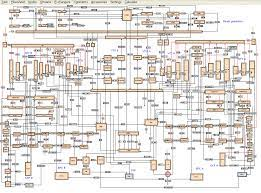
\includegraphics[width=0.75\textwidth]{figuras/RECONSET.jpg}
        \caption{Tela Principal da ferramenta RECONSET.}
        \vspace{6mm}
        \label{fig:RECONSET}
    \end{center} 
\end{figure}

O \textit{software} é orientado para PC e possui uma interface de usuário gráfica interativa, tornando-o fácil de usar. Os usuários definem problemas (ou tarefas) interativamente por meio desta interface. O RECON é capaz de equilibrar materiais e energia de componentes únicos ou múltiplos de sistemas complexos, seja em estado estacionário ou instável (dinâmico), com ou sem reações químicas (balanceamento de reatores). Além disso, ele pode realizar balanceamento de momento com base em cálculos hidráulicos de vazão em sistemas de dutos. O RECON reconcilia vazões medidas, concentrações, temperaturas e outras variáveis de processo, e calcula variáveis não medidas. Para definir um problema (ou tarefa), os usuários geralmente criam um fluxograma de processo e definem variáveis de processo, como taxas de fluxo, temperaturas, pressões, etc. O fluxograma inclui nós, fluxos de massa e energia, e trocadores de calor. Se necessário, os usuários também podem complementar (ou até mesmo substituir) o modelo de balanceamento com suas próprias equações.

\subsubsection{BILCO}

CASPEO é uma empresa francesa fundada em 2004, especializada em engenharia de processos e soluções tecnológicas. Originada do 
Departamento de Pesquisas Geológicas e Minerais da França. Ela foi criada para oferecer à indústria de mineração métodos e ferramentas computacionais resultantes de anos de pesquisa e tornou-se uma referência na indústria de processamento mineral, atendendo a vários mercados, como mineração e metalurgia, processamento de biomassa e alimentos, tratamento de resíduos sólidos e outras indústrias de processamento \cite{bilco}.

Uma das suas inovações é o \textit{software} de reconciliação de dados BILCO, projetado para derivar um balanço de material coerente e total a partir de todos os dados disponíveis (medições, análises, estimativas) para todas as correntes de processo. Ele é uma ferramenta poderosa que permite aos usuários reconciliar dados de qualquer planta de processamento, a Figura \ref{fig:BILCO}, demonstra a tela inicial do \textit{software}.

\begin{figure}[htbp!] 
    \begin{center}
        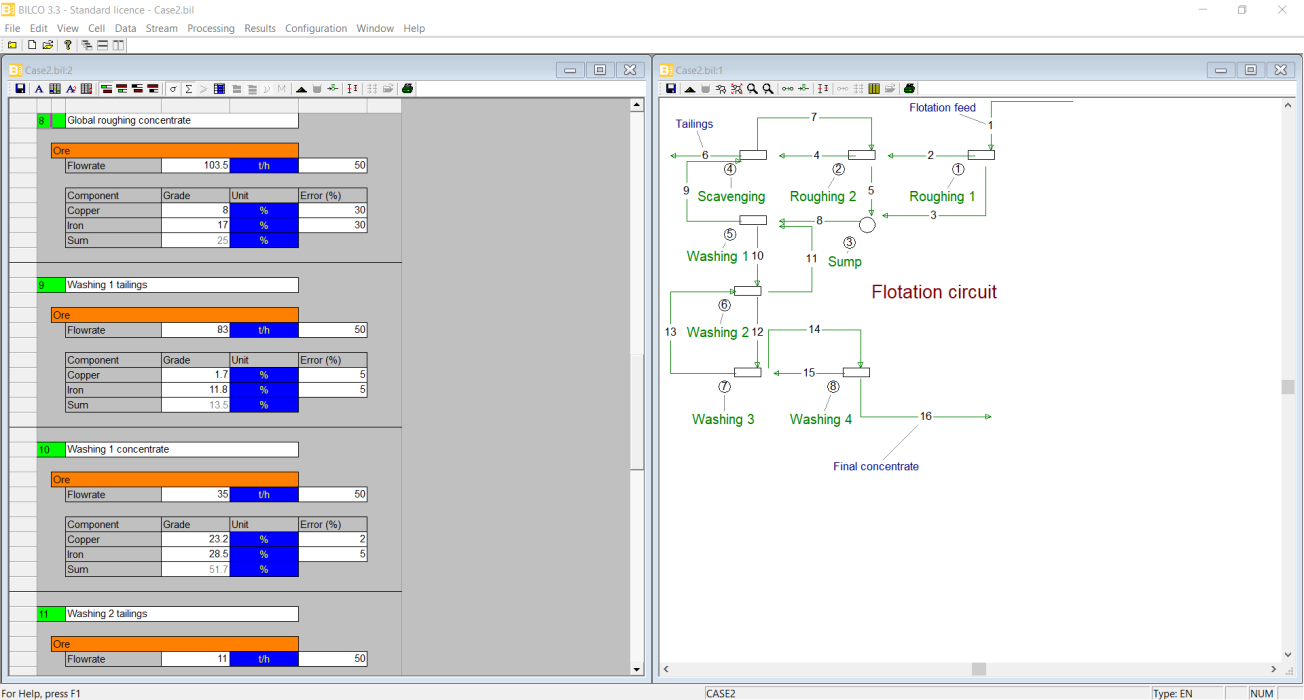
\includegraphics[width=0.75\textwidth]{figuras/BILCOCASPEOP.png}
        \caption{Tela Principal da ferramenta BILCO.}
        \vspace{6mm}
        \label{fig:BILCO}
    \end{center} 
\end{figure}

Ele tem a capacidade de se incorporar à duas outras ferramentas facilmente, no caso, à um simulador de processos, denominado USIM PAC e à um \textit{software} de contabilidade metalúrgica, INVETEO; e, dessa forma, fornece cálculos de balanço precisos e gera um conjunto de estimadores coerentes que estão em conformidades com as restrições da lei de conservação de energia, além de calcular seus erros relativos. Ele também é capaz de determinar, em quantidade e qualidade, a composição de cada corrente de processo. É um dos poucos \textit{softwares} de balanço de massa capaz de calcular toda a composição da corrente (taxas de fluxo, classes de tamanho, tipos de partículas, massa molar, etc.) em um único cálculo.

Essa solução também oferece uma única interface para gerenciar todo o processo. Consiste numa interface gráfica fácil de usar, tornando-a acessível tanto para novos usuários quanto para os mais experientes. Uma das características mais úteis do BILCO é a possibilidade de exportar os resultados para o Excel, permitindo uma análise mais profunda dos dados. Ele fornece resultados detalhados, incluindo uma planilha de comparação e uma planilha global, para uma visão completa do balanço de material.

\subsubsection{PIMSOFT}

Shorou International é uma empresa dos Emirados Árabes Unidos, que oferece soluções especializadas e serviços de engenharia com foco em automação avançada e gestão de ativos para todas as principais indústrias, com ênfase especial nos setores de petróleo, gás, utilidade e energia \cite{pimsoft}.

Uma das suas soluções é o Sistema OSIsoft PI, uma plataforma que coleta, historiza e analisa grandes quantidades de dados de séries temporais, de alta fidelidade, de várias fontes de dados e em diferentes formados. Esses dados são disponibilizados para usuários e sistemas em diversos setores de negócios. As implementações do sistema PI aproveitam o poder dos dados operacionais para gerar previsões que aumentam a consciência situacional e desencadeiam decisões bem planejadas, ajudando as empresas líderes a alcançar maiores melhorias operacionais e inovações revolucionárias em seus respectivos campos. 

E um complemento desse sistema, é o PIMSOFT SigmaFine que é um \textit{software} de verificações e balanços que utiliza princípios de conservação, estatísticas, padrões de engenharia e cálculos para monitorar e montar dados de plantas industriais. SigmaFine gera módulos coerentes, confiáveis e utilizáveis, prontos para negócios.

\subsection{Aplicação na Contabilidade}

Paralelamente à disciplina de Reconciliação de Dados na área industrial química, há uma outra área na qual investe bastante nesse campo, a de soluções contábeis. E a investigação das tendências tecnológicas emergentes é um aspecto crucial durante o processo de desenvolvimento de uma solução mais dinâmica e que consegue resolver problemas já solucionados por outras áreas da ciência.

\subsubsection{FloQast}

FloQast é uma empresa fundada em 2013, que possui uma plataforma  de contabilidade operacional baseada na nuvem, com foco em automação e gestão para uso por contadores. Uma das suas soluções é uma ferramenta de reconciliação de dados nomeada FloQast Reconciliation Management, uma solução avançada de automação de fluxo de trabalho para fornecer gerenciamento de reconciliação de contas de ponta a ponta \cite{floqast}.

Isso aumenta a velocidade e a precisão financeira do fechamento financeiro, ao mesmo tempo que gerencia o risco de declaração incorreta. Esse \textit{software} permite que controladores e suas equipes automatizem e gerenciem o processo de reconciliação de ponta a ponta, com uma solução centralizada confiável por contadores e auditores em todo o mundo.

\subsubsection{Aspen}

AspenTech, uma empresa fundada em 1981, a partir do Projeto ASPEN - uma pesquisa conjunta entre o MIT (Instituto de Tecnologia de Massachusetts) e o Departamento de Energia dos EUA na qual desenvolveu a primeira tecnologia de modelagem e simulação baseada em computador para a indústria química. Hoje, mais de 40 anos depois, com mais de 3700 funcionários e 60 localidades em todo o mundo, a empresa tem seu foco em soluções industriais, ao mesmo tempo em que enfrenta diretamente a sustentabilidade, com foco na eficiência dos recursos, transição energética, descarbonização e redução de resíduos \cite{aspen}.

Uma das suas ferramentas que utiliza soluções similares às do trabalho de conclusão de curso é a ferramenta AURA (Aspen Unified Reconciliation Accounting) uma solução que ajuda a reduzir perdas de material e aumentar margens por meio de um equilíbrio eficiente de massa e volume. Capacitando as partes interessadas a tomar melhores decisões com base em dados de produção validados e reconciliados. Sua arquitetura escalável reduz o custo total de propriedade com opções rápidas de implantação na nuvem e fácil implementação e manutenção do modelo. A precisão da reconciliação é aumentada pelo \textit{Smart Solver} proprietário que resolve automaticamente os erros de densidade medidos em laboratório. O \textit{software} também ajuda a atingir metas de redução de emissões ao automatizar o rastreamento, monitoramento e relatórios de emissões de gases de efeito estufa e intensidade de carbono do produto. Além disso, permite fechar o balanço mais rapidamente com fluxos de trabalho intuitivos, interpretação fácil dos resultados com visualização avançada e relatórios dinâmicos poderosos.


% ---

\subsection{Pesquisas Sendo Desenvolvidas}

O objetivo do RADARE é incorporar avanços tecnológicos de diversas áreas, com foco não apenas nas técnicas aplicadas diretamente à reconciliação de dados, mas também em áreas adjacentes que possam contribuir para o aprimoramento da ferramenta. Dessa forma, é fundamental estar alinhado com as pesquisas mais recentes em reconciliação de dados computacional, bem como explorar como elas podem ser aplicadas no contexto industrial brasileiro.

Pesquisas em outras áreas de aplicação, como o processamento mineral e a distribuição de gás, também oferecem contribuições valiosas para o desenvolvimento do RADARE, especialmente na aplicação de técnicas de reconciliação de dados em diferentes cenários industriais.

\subsubsection{Controle e Supervisão de Processamento Mineral}

A pesquisa apresentada por Daniel Hoduin \cite{danielhoduin} foca nas restrições de conservação de massa e energia, que servem como base para o desenvolvimento de estratégias de medição, atualização do valor medido por meio de técnicas de filtragem de erros de medição e estimativa de variáveis de processo não medidas. Nas unidades de processamento mineral, as principais variáveis são geralmente as vazões e concentrações, e a reconciliação desses dados com as leis de conservação de massa é essencial para manter a precisão dos processos.

Os métodos de reconciliação propostos utilizam técnicas clássicas, como os mínimos quadrados usuais, que minimizam os erros entre os valores observados e os valores estimados. Além disso, a filtragem de Kalman, um algoritmo de estimação recursiva, é empregada para estimar variáveis de estado de processos dinâmicos e com ruído. São sugeridas ferramentas para três tipos de regimes operacionais: regime estacionário, quase-estacionário e dinâmico.

As ferramentas propostas para diferentes regimes operacionais de processamento mineral podem ser adaptadas para o RADARE, permitindo que ele lide com cenários variáveis de fluxo de dados e oferecendo maior flexibilidade no tratamento de dados de processos industriais com características dinâmicas.

\subsubsection{Balanços de Materiais em Rede de Distribuição de Gás}

O desenvolvimento realizado por Jesús David Badillo Herrera, Arlex Chaves e José Augusto Fuentes Osorio \cite{balancecontrol}, foca em uma solução prática para enfrentar os desafios apresentados por erros em sistemas de distribuição de gás natural. A ferramenta combina técnicas numéricas e estatísticas, como a Reconciliação de Dados (DR) e a Detecção de Erros Brutos (GED), para melhorar a precisão das medições e garantir a conformidade com as leis de conservação de massa.

Essa abordagem não apenas aprimora a acurácia das medições, mas também identifica e corrige erros grosseiros, proporcionando maior confiabilidade nos dados. A validação da ferramenta com problemas da literatura e sua aplicação em uma rede de distribuição real demonstram sua eficácia em fornecer resultados reconciliados com alta precisão.

A abordagem combinada de Reconciliação de Dados (DR) e Detecção de Erros Brutos (GED), utilizada na distribuição de gás natural, foi ser integrada ao RADARE para garantir maior precisão nas medições e identificar rapidamente inconsistências ou erros em sistemas industriais.

% ---

\section{Justificativa}

O setor industrial brasileiro, responsável por uma parcela significativa da economia nacional, enfrenta desafios críticos relacionados à qualidade e confiabilidade dos dados gerados em processos produtivos. A falta de precisão nas medições e a ausência de ferramentas eficazes para a reconciliação de dados comprometem a eficiência operacional e a competitividade das indústrias. Dessa forma, torna-se urgente o desenvolvimento de soluções tecnológicas que possam superar essas limitações, sendo o \textit{software} RADARE uma proposta que visa preencher essa lacuna com inovação e eficácia.

A escolha por desenvolver o RADARE como uma aplicação \textit{web} é estratégica, pois o ambiente web oferece diversas vantagens essenciais para o setor industrial. Entre elas, a interoperabilidade eficiente entre sistemas permite integrar o \textit{software} com outras ferramentas já utilizadas nas plantas industriais. O acesso remoto possibilita que engenheiros e operadores possam monitorar e controlar os processos de qualquer localidade, reduzindo tempos de inatividade e melhorando a resposta a problemas. Além disso, a facilidade de uso da plataforma, associada à alta acessibilidade para indivíduos com necessidades especiais, amplia o alcance da solução, garantindo que o sistema possa ser adotado por uma gama diversa de usuários.

O projeto RADARE visa atender a uma demanda crescente por soluções no setor industrial brasileiro, onde a competitividade global exige maior eficiência e qualidade nas operações. O contexto brasileiro apresenta desafios específicos, como a falta de ferramentas acessíveis e adaptadas à realidade das indústrias locais. O RADARE se diferencia por ser uma solução criada para o contexto nacional, ao mesmo tempo em que incorpora tecnologias de ponta e metodologias comprovadas internacionalmente, como o método dos multiplicadores de Lagrange, aplicado de forma inovadora em uma plataforma web de fácil acesso e integração.

O RADARE representa uma inovação ao unir teorias avançadas de reconciliação de dados com tecnologias modernas de desenvolvimento \textit{web}. Ao criar uma solução que é tanto acessível quanto adaptável às necessidades do setor industrial, o RADARE tem o potencial de impactar diretamente a eficiência das operações industriais no Brasil, promovendo o desenvolvimento tecnológico e aumentando a competitividade das empresas brasileiras no cenário global.

Este trabalho está estruturado da seguinte forma: no Capítulo 1, apresenta-se a introdução, contextualizando o problema e destacando os objetivos principais e secundários da pesquisa. O Capítulo 2 oferece o referencial teórico, com definições e descrições das principais teorias que embasam a solução proposta. No Capítulo 3, descrevem-se os métodos e técnicas utilizados para o desenvolvimento do sistema, assim como o cronograma de atividades apresentado por meio do diagrama de Gantt. Por fim, no Capítulo 4, são feitas as considerações finais sobre o aprendizado adquirido, as reflexões sobre os resultados esperados no desenvolvimento futuro do projeto e as contribuições gerais da pesquisa.
